\chapter{Methodology and Experimental Setup}
\label{chap3}
% \thispagestyle{fancy}
\textit{This chapter motivates the methodologies to address the research questions while incorporating engineering subject matter, such as models, hardware platforms, and software environments pertinent to this degree project.} 

\section{Modelling}
The process of modeling a robot is a fundamental step in developing an effective controller. Modeling soft-legged robots with soft actuators is challenging due to the non-linearity, time-variant properties, and unpredictable behaviors of soft materials. Despite these difficulties, research groups from KTH Royal Institute of Technology\cite{jiSynthesizingOptimalGait2022, daneliaStructureGaitOptimizationof2021, thorapallimuralidharanContinuumActuatorBased2020, jiLearningbasedControl4D2022} have successfully constructed a soft quadruped robot using soft continuum actuators, enabling it to walk. However, the robot's movement is not yet optimal, emphasizing the necessity for continued research and development in this field. This thesis work was based on this complete soft quadruped robot model, SoftQ, which is shown in Fig. \ref{fig:robot}(a). 

\subsection{Physical Model}
SoftQ is a tendon-driven and lightweight robotic system that capable of locomotion similar to quadruped animals. The physical body of SoftQ is comprised of discrete subsystems, each playing a pivotal role in its operational intricacy. At its core, the robot's main body assumes the form of a hollow lightweight panel, housing an array of essential constituents, including servo motors, STM32 microcontroller, Raspberry Pi, electrical interface board, voltage converter, \ac{IMU} sensor, \ac{ToF} sensors, batteries, and complex wiring infrastructure. The servo motor plays a pivotal role by transducing pulse signals into rotational torque via its shaft, subsequently translating this torque through a spool mechanism onto a connected tendon string. This interaction engenders the generation of tendon force, which is then transmitted to the actuator to induce controlled deformation. The deformation process is guided by the equilibrium between the applied tendon force and the reactive force exerted by the actuator. Because of the morphology of actuation systems, the whole actuator is so called \ac{CTSA} and the details are illustrated in \ref{fig:robot}(b)-(d). The robot's locomotion is enabled by these four \ac{CTSA}s that are strategically grouped and positioned to govern the movement of individual legs, and each leg is actuated by three motor and \ac{CTSA} systems. \begin{figure}[htb]
    \centering
    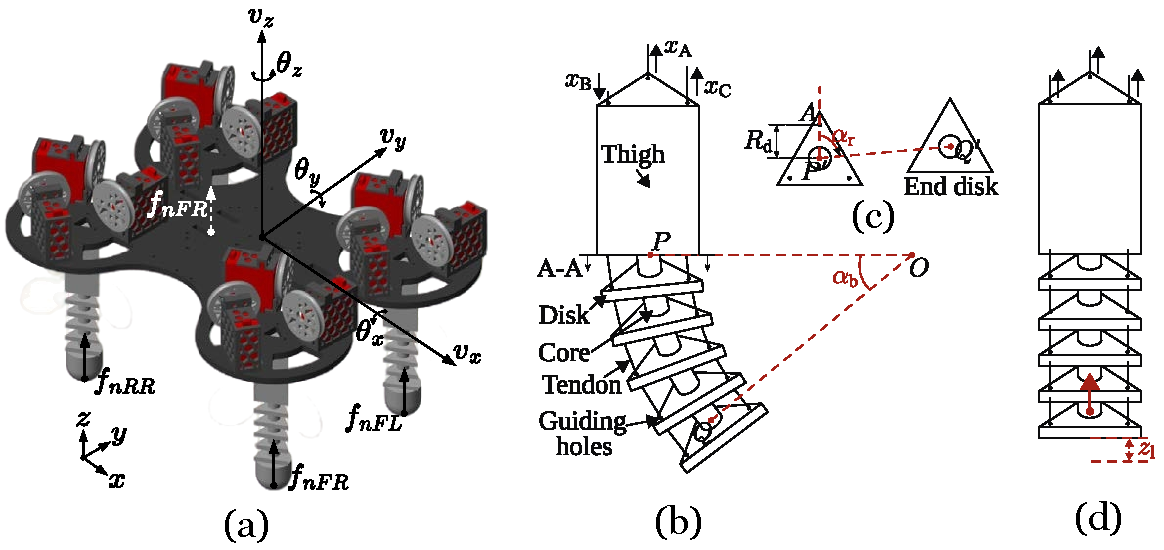
\includegraphics[width=\linewidth]{img/chap3/robots.pdf}
    \caption{Graphical overview of SoftQ and the Compressible Tendon-driven Soft Actuator (CTSA) to drive the robot. (a) Rendered robot with key state notations. (b) The structure and notations of the CTSA. The upper part from section A-A is the rigid thigh for maintaining the actuator length and the lower part is compressible and bendable. The bending angle of the lower part is noted as $\alpha_b$. (c) The top view of the bent CTSA of section A-A. $\alpha_r$ refers to the rotational angle of the CTSA. (d) The CTSA compression is realized by pulling the three tendons by the same amount, with the compression length being noted as $z_l$, originated from Ji et al.\cite{jiSynthesizingOptimalGait2022, jiOmnidirectionalWalkingQuadruped2022}}
    \label{fig:robot}
\end{figure} Notably, the \ac{CTSA}s present a pioneering feature of SoftQ, encompassing soft continuum actuators that facilitate continuous bending or twisting motion throughout their length. Through three motor and \ac{CTSA} systems that evenly distribute forces at radial locations, the robot's four legs attain the capacity for versatile omnidirectional bending\cite{jiOmnidirectionalWalkingQuadruped2022}. Between the \ac{CTSA} and the foot, sensory feedback of contact force is furnished by force sensors attached between them, detecting forces resulting from ground contact, depicted in Figure \ref{fig:actuation}(d). The electrical interface board plays a vital role in this robotic system, facilitating the transmission of both signals and power among motors, microcontrollers, and power sources. Beneath this board, a Raspberry Pi is plugged and mounted by screws, while seamlessly integrated upon it are a STM32 microcontroller and an \ac{IMU}. Additionally, \ac{ToF} sensors are strategically positioned in varying orientations via external hubs, enabling multi-directional sensory input. Accompanying these components, voltage converters and batteries find their placement beneath the panel. Through interconnecting cables, they provide power to the servo motors via the interface board. This distinctive mechanism is visually demonstrated in Figure \ref{fig:robot}, effectively showcasing the robot's versatile and agile locomotion capabilities.

Of particular significance, the architecture of the \ac{CTSA} entails a sequential arrangement of rigid disks and flexible cores, the details of actuation are illustrated in Fig. \ref{fig:actuation}. The interface between the servo motor's shaft and a connected spool serves to convert motor torque into tendon-based force. The end of the tendon are tethered to the spool and the terminal disk of the contiguous continuum structure. Rotation of the spool induces a corresponding change in tendon length. The central position of the spool, designated as position 0, corresponds to the neutral configuration where the actuator assumes a linear form. Positive spool rotations induce tendon retraction, while negative rotations become slack. Tendon-induced forces elicit actuator deformation, with the balance between tendon force and actuator reaction force governing deformation dynamics. The three driven tendons adopt a radial distribution around the actuator's rigid disks, passing through guiding apertures on said disks. The length of the actuators with core and disk structures has been modified, with the upper thigh region reinforced to enhance rigidity. The guiding apertures on rigid disks enable unfettered tendon motion while maintaining positional stability, as depicted in Figure \ref{fig:robot}. This specific attribute eliminates the requirement for discrete joints or segments, thereby contributing to the robot's innate flexibility and agility. To achieve optimal actuator bending while preserving overall robot balance, the servo motor's maximum rotational angle is capped at $\bar{a}_M = \pi/6$, corresponding to a rotational range of [-$\bar{a}_M$,$\bar{a}_M$]. This angular range corresponds to a \ac{PWM} signal interval of [6.67\%, 8.33\%].
\begin{figure}[ht]
    \centering
    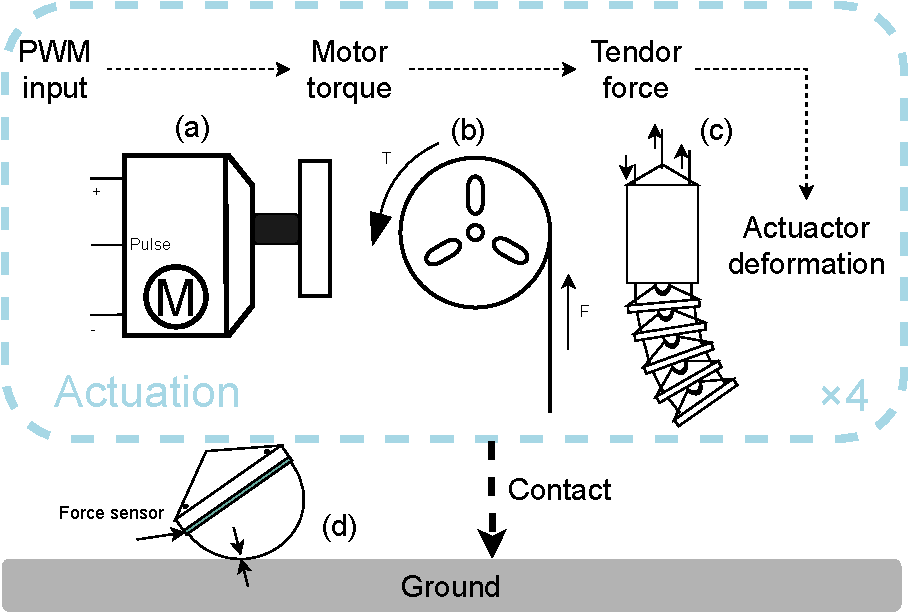
\includegraphics[width=0.9\linewidth]{img/chap3/actuation.pdf}
    \caption{Overview of the quadruped robot's main subsystems enabled by tendon-driven soft actuators. (a) Servo motor converts PWM signal to rotational motions while applying torque exerted on the rotational spool. (b) The spool translates the torque from the servo motor to the traction force in the tendon. (c) The tendon force is applied on the actuator and effectuates its deformation. (d) The actuator's deformation introduces relative motion between the robot's feet and diverse ground conditions, thereby instigating the overall locomotion of the quadruped robot. Reproduced from Ji et al.\cite{ji2022Synthesizing, ji2022Omnidirectional}}
    \label{fig:actuation}
\end{figure}


Furthermore, the inverse kinematics model of \ac{CTSA} using three tendons can be derived through geometric analysis as discussed in \cite{muralidharanSoftQuadrupedRobot2021}, and is expressed as follows:
\begin{equation}
    \begin{aligned}
    x_A &= R_d\alpha_b\cdot{\cos(\alpha_r)} \\
    x_B &= R_d\alpha_b\cdot{\cos(\alpha_r+\frac{2}{3}\pi)} \\
    x_C &= R_d\alpha_b\cdot{\cos(\alpha_r+\frac{4}{3}\pi)}
    \end{aligned}
    \label{eq:value2motor}
\end{equation}

Here, $x_{A,B,C}$ denote the tendon displacement. The positive values of $x_{A,B,C}$ indicate that the tendon pulls the respective actuator end, while negative values signify tendon release and slackening. $R_d$ represents the radius of the circle formed by the three guiding holes on a disk as depicted in Figure \ref{fig:robot}(b). The geometric correlation between $[\alpha_b, \alpha_r]^T$ and $[x_A, x_B, x_C]^T $ can be encapsulated as a function: $g: \mathbb{R}^2 \rightarrow \mathbb{R}^3$. For the described \ac{CTSA}, assuming that the compressed length of the actuator $z_l$ results solely from equal-length pulling of the three tendons, the actuator's total degrees of freedom are established as three: $[\alpha_b, \alpha_r, z_l]^T$. Consequently, the inverse kinematic model of the \ac{CTSA} becomes $f : \mathbb{R}^3 \rightarrow \mathbb{R}^3$:
\begin{equation}
    \begin{bmatrix}x_A\\x_B\\x_C\end{bmatrix} = f(\begin{bmatrix}\alpha_b\\ \alpha_r\\ z_l\end{bmatrix}) = g(\begin{bmatrix}\alpha_b\\ \alpha_r\end{bmatrix}) + z_l\begin{bmatrix}1\\1\\1\end{bmatrix}
    \label{eq:cov2eq}
\end{equation}

The SoftQ is a sophisticated robot for this project, and only part of sensors will be used to guide the optimal gait controller design. The servo motor interfaces with \ac{PWM} signals, generating rotational torque  that is subsequently propagated to downstream subsystems. The utilized servo motor is TS-411MG model from TrackStar, which receives \ac{PWM} signals and rotates the shaft proportionally by a built-in position controller with corresponding sensors. In specific, the robot's feet are equipped with four force sensors each, labelled as \ac{FR}, \ac{FL}, \ac{RR}, and \ac{RL2}. Constituting the sensing suite are five \ac{ToF} sensors from the Adafruit VL53L1X series strategically positioned to measure distances from various sides, including the front, back, left, and right sides, as well as the bottom of the robot. Additionally, an \ac{IMU} module sourced from Adafruit BNO055 is centrally mounted to facilitate the detection of the robot's pose and localization. For precise localization, the outputs of the \ac{ToF} sensors are fused with the robot's rotational and translational accelerations, as quantified by the \ac{IMU}. This sophisticated data fusion strategy culminates is developed in this thesis for the robot to accurately discern its position and orientation. This augmentation proves particularly advantageous for the successful implementation of \ac{MBRL}. Particularly, certain sensors such as optical cameras and current sensors dedicated to motor control have been mounted on the robot but have not been integrated into the system. This deliberate omission stems from the focused scope of this thesis, which primarily centers on lower-level control aspects and gait coordination.

In order to facilitate the gait control of SoftQ, the robot's local coordinate system has been established utilizing the conventions of the right-hand rule, which is shown in Fig.\ref{fig:robot}(a). In this frame of reference, the $x$ direction denotes the frontal orientation, while the anti-gravity direction aligns with the $z$ direction. For capturing the robot's movements, the roll, pitch, and yaw motions are depicted through the rotational angles of the body center encompassing the three orthogonal axes, designated as $\theta_x$, $\theta_y$, and $\theta_z$. The translational moving velocities are also represented by the movement of the body center in the three directions and are noted as $v_x$, $v_y$ and $v_z$, respectively.

\subsection{Modeling in MathWorks Simulink\texorpdfstring{\textsuperscript{\textregistered}}{(R)}}
\label{sec3.2}
The Simulink model of SoftQ comprises multiple interconnected subsystems, each serving a distinct purpose. These include the motor-driven units, the tendon transmission mechanism, the flexible structure deformation system, and the ground contact subsystem. To model servo behavior in simulation, a \ac{PWM} signals was employed to control the motor, attaching a spool and varying loads and adjusting servo parameters until the deviation between the experimental and the simulation data is minimal. 

As visually depicted in Fig. \ref{fig:robot}, the \ac{CTSA} is constructed through a sequential combination of flexible cores and rigid disks with triangle shapes to retain a high stability and fast fabrication. The three driven tendons are equally distributed at a radial formation around the rigid disks and passed through respective guiding holes placed on the rigid disks, and through the cooperation of three tendons deformation, the legs could realize omnidirectional movement. To model the above soft actuator deformations, the lumped parameter method was applied, where rigid components are applied to build the shape of the cores and the disks while using spring and damper joints for modeling the connections between the cores and disks and enabling the target bending and compression actuator motions. These joints use equivalent stiffness and damping to provide equal response of the entire actuator compared with the flexible segments, only needs to estimate the rigid connecting joint motions with stiffness $k$ and damping $d$ properties in the bending and longitude directions, denoted as $k_B$, $d_B$, $k_L$ and $d_L$ respectively. In the MATLAB Simscape Multibody environment, the continuum structure was modelled using rigid components with telescope joints. Through a series of simulation trials, the equivalent bending properties were estimated to $k_B = 0.0005 N m/deg$ and $d_B = 0.00002 N m/(deg/s)$, and the longitude stiffness and damping were estimated as $k_L = 15000 N/m$ and $d_L = 800 N/(m/s)$.

The tendons simulation was modelled using a belt-cable function within the MATLAB Simscape Multibody environment. This block facilitated a direct connection with the spools and foot, omitting pulleys between the holes on the rigid disks for simulation efficiency. However, recognizing the variance introduced by this omission, a corrective coefficient, $\alpha_c = 1.16$, was introduced. This coefficient adjusts the servo motor's commanded rotation angle ($\theta$) by multiplying it with $\alpha_c$, aiming to bring the actuator's behavior in closer alignment with experimental observations. Furthermore, the use of continuum actuators in the robot, particularly the inclusion of the thigh segment, without the use of pulleys to secure tendon positions, introduces increased model errors due to the simulated detachment of tendons from the thighs. To overcome this issue, adjustments were made by relocating the spools on the servo motor shafts to the lower section of the thigh. This repositioning effectively prevents the tendons from exiting the thigh structure and consequently reduces the model error associated with the lack of pulley configurations. 

The robot is placed on the ground with gravitational forces in the simulation environment. The diverse motions of the four legs result in relative movement with the ground, generating static or dynamic friction that propels the robot's overall movement. It is important to acknowledge that the distinct frictional properties of different ground conditions can lead to varied robot motions. To model the interaction between the quadruped robot's feet and the ground, static and dynamic friction coefficients were specifically determined as $f_s = 0.315$ and $f_d = 0.3$ respectively.

The update period of the RL algorithm is $T_s = 0.05s$ and the simulation model of the soft robot is a continuous-time model. The robot's state representation consists of ten key parameters: the roll, pitch and yaw rotations ($\theta_x$, $\theta_y$, $\theta_z$), translational moving velocities in three axis ($v_x$, $v_y$, $v_z$) and contact force on each feet ($f_{nFL}$, $f_{nFR}$, $f_{nRR}$, $f_{nRL}$). To prevent the robot from falling down or entering unstable states in which the simulation results would be unreliable, termination boundaries are set in the simulation environment. When the robot states meet these termination conditions, the simulation ends before the desired simulation time. The roll and pitch angles of the body center $\theta_x$ and $\theta_y$, are set to rotate less than 0.15 rad, while the bending angle $alph_b$ of all the four legs are set to less than $\pi/3$ rad. 

\section{Experiment Setup}
The experimental setup for MBRL of the SoftQ quadruped robot encompasses a comprehensive integration of hardware and software components to facilitate the training and evaluation of the robot's locomotion control policies. The SoftQ robot, equipped with its sophisticated subsystems as described earlier, serves as the physical platform for conducting the experiments. 

\begin{figure}[ht]
    \centering
    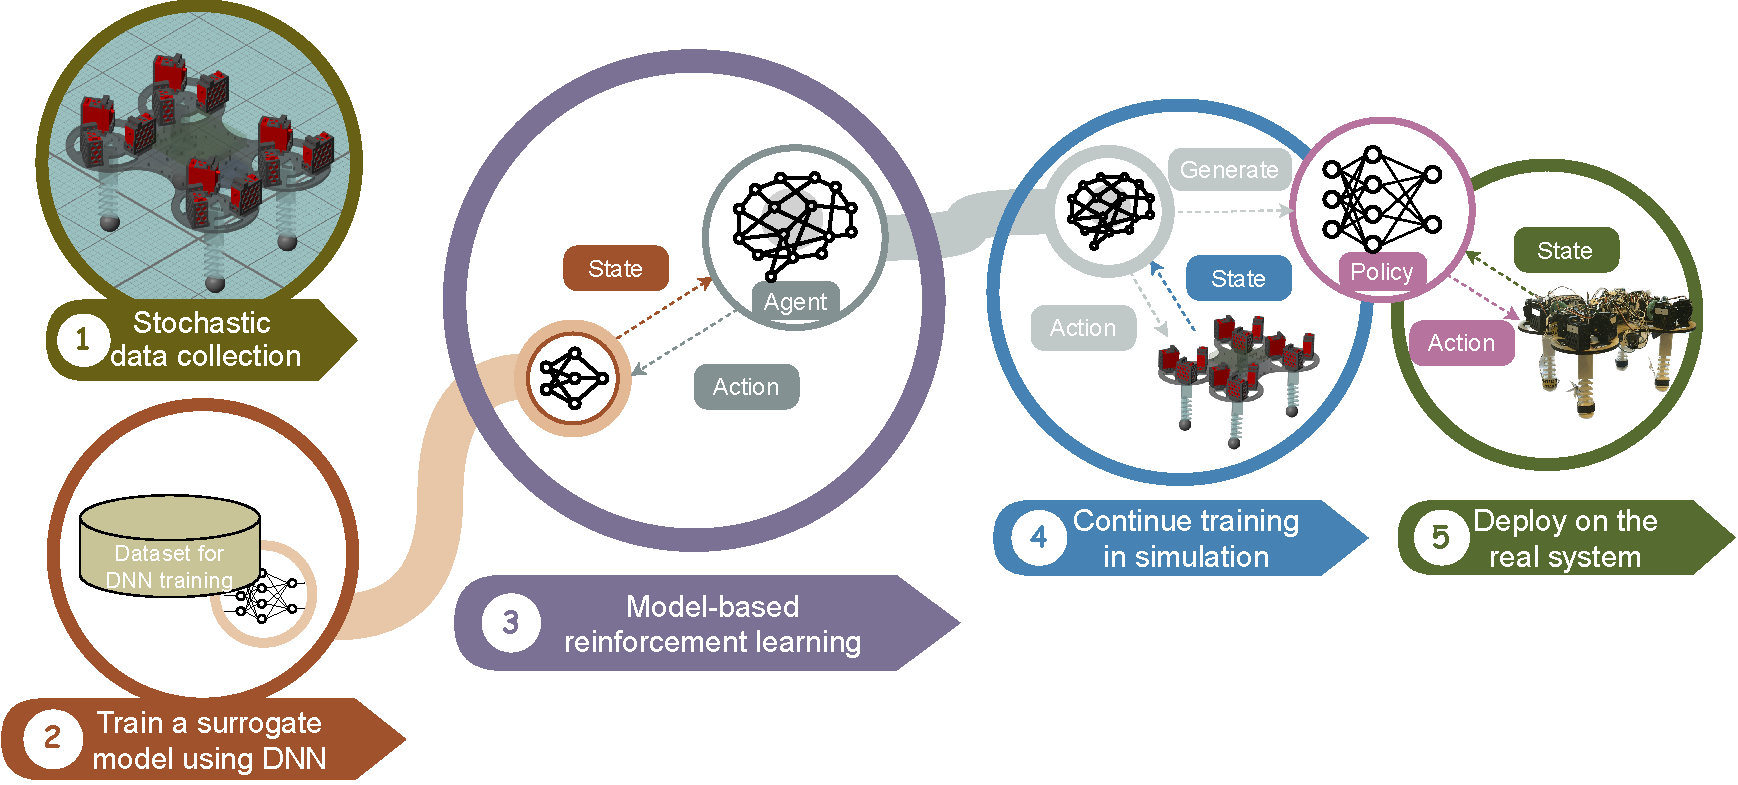
\includegraphics[width=\linewidth]{img/chap3/experiment.pdf}
    \caption{Creating a gait control policy. In the initial step, the physical parameters of the robot was identified and the stochastic actions were simulated in the identification to collect the data. In the subsequent step, an action-observation net was train that models complex robot model dynamics. The third step capitalized on the surrogate models produced in the previous two steps to train a control policy. In the fourth step, the trained control policy was further refined in simulation before deploying on the physical system.}
    \label{fig:exp}
\end{figure}



In this thesis, a practical methodology for autonomously learning and transferring agile and dynamic motor skills for complex and large legged systems were developed. This experimental framework constitutes a pivotal contribution to the field, encapsulated in the schematic representation shown in Figure \ref{fig:exp}. The central premise of this study revolves around the utilization of \ac{RL} to train the gait controller through trial and error, which involves creating a virtual model of the robot and its environment to simulate possible walking behaviors and test the efficacy of various control policies. This approach is motivated by the challenges associated with collecting data in the physical world, which can be time-consuming, costly, and hazardous. By leveraging the benefits of simulation, the training process can generate a large volume of data quickly and inexpensively, allowing for the exploration of a broad range of behaviors and control policies without exposing the physical robot to potential risks.

Central to our approach is the utilization of a surrogate model to facilitate the training of controllers via the principles of deep neural network. This surrogate model serves as a vital intermediary in the training pipeline, mediating the interaction between the RL algorithm and the complex robotic system models. The architecture of surrogate model is embodied in a multi-layer perceptron, which operates as a neural network capable of capturing intricate relationships within the data. This multi-layer perceptron is engineered to process the potential sequence of the robot's states as input and subsequently generate the corresponding actions to be executed by legs as output. This architectural configuration enables the controller with the ability to encapsulate a wide array of state-action dependencies, thereby fostering expedited controller training. Preceding the training of the surrogate model, the collection of stochastic actions and their associated observations is requisite. This data collection process can be time-intensive, but its advantages extend to its reusability for the training of other controllers. This data-driven approach allows for efficient iteration and optimization of the training process, resulting in a control policy that can be effectively applied to the robot.

The trained controller, obtained from the \ac{MBRL} paradigm, would then proceed to a subsequent phase of refinement within the simulation environment. This phase entails simulation-based continuous training, which augments the controller's robustness and efficacy, thereby reducing the reality gap and enhancing its adaptability. Subsequently, the controller that has been refined in the virtual domain is seamlessly transitioned to the physical robotic system. This direct deployment showcases the transferability and generalization capabilities of the acquired motor skills, as the controller is able to translate its learned behaviors from simulation to the tangible real-world setting.

This methodology facilitates the application of deep learning and reinforcement learning techniques to develop a robust and efficient gait controller for the soft quadruped robot. The MATLAB functions developed and Simulink blocks constructed primarily utilize the CPU. The details of control architecture and the model-based reinforcement learning framework will be shown in the next chapter. During experimentation, the robot undergoes iterative training episodes, where it interacts with its environment to learn locomotion policies. The development environment is listed in Table \ref{tab:env}. Thanks to efficient software implementations, no special computing hardware was needed, such as multi-CPU or multi-GPU servers, for training. All training sessions presented in this thesis were done on a personal computer with one CPU and one GPU, and none lasted more than twenty hours.
\begin{table}[ht]
    \centering
    \begin{tabular}{ll}
        \toprule
        Component        & Description                             \\\midrule
        Operating System & Windows 10                              \\
        \ac{IDE}              & MATLAB R2021b                           \\
        \ac{CPU}              & Intel(R) Core(TM) i7-4770 CPU @ 3.40GHz \\
        Memory           & 16 GB                                   \\\bottomrule
        \end{tabular}%
    \caption{Development environment for stochastic model}
    \label{tab:env}
\end{table}


The collaboration of these hardware elements significantly enhances both the robot's operational capabilities and its potential for learning. A concise depiction of these hardware constituents is aptly captured in Table \ref{tab:board}, highlighting pivotal components including servo motors, motor control boards, high-level control boards, interface boards, \ac{IMU} units, \ac{ToF} sensors, step-down regulators, and batteries. These components collectively contribute to the robot's ability to perceive its surroundings, execute precise movements, manage power, and establish connections with the external world. It gives rise to a comprehensive robotic system, primed to dynamically interact with its environment and gradually enhance its locomotion capabilities through the exploration of model-based reinforcement learning techniques. In the next chapter, which includes details about control architecture and learning frameworks, the alignment between these hardware components and the research objectives becomes increasingly evident.
\begin{table}[htbp]
    \centering
    \begin{tabular}{lp{10cm}}
        \toprule
        Component        & Description                             \\\midrule
        Servo motor$\times 12$  & TrackStar TS-411MG  (Information from: \href{https://hobbyking.com/en_us/trackstar-ts-411mg-digital-1-10-scale-short-course-steering-servo-11-1kg-0-09sec-57g.html?___store=en_us}{HobbyKing.com}) \\
        Motor control board & STM32G431KB (Information from: \href{https://www.st.com/en/evaluation-tools/nucleo-g431kb.html}{st.com}) \\
        High level control board  & Raspberry Pi4 Model-B standard (Information from: \href{https://www.raspberrypi.com/products/raspberry-pi-4-model-b/}{raspberrypi.com}) \\
        Interface board & Designed by Muralidharan et al. \cite{thorapallimuralidharanContinuumActuatorBased2020} and manufactured by Shenzhen JLC Technology Group Co., Ltd \\
        \ac{IMU} & Adafruit BNO055 9-DoF@I2C (Information from: \href{https://www.bosch-sensortec.com/products/smart-sensors/bno055/#documents}{Adafruit.com}) \\
        \ac{ToF} $\times 5$ & Adafruit VL53L1X Breakout (Information from: \href{https://www.mouser.se/ProductDetail/Pimoroni/PIM373?qs=lc2O%252BfHJPVbu7kI%2FlA0xSg%3D%3D}{mouse.com}) \\
        Step down regulator & LTC3780 DC-DC 5-32V to 1V-30V 10A (Information from: \href{https://www.analog.com/en/products/ltc3780.html#product-overview}{analog.com}) \\
        Battery $\times 2$  & Li-PO 2S 7.4V 30C 1300mAh  (Information from: \href{https://www.batteriexperten.com/sv/artiklar/li-po-2s-74v-30c-1300mah-t-kontakt-vapex.html?gclid=CjwKCAjwoqGnBhAcEiwAwK-OkaSSg7U-01roWZIcyx2yhCrvc7GKyWF5eUhzEE2re9kqi-mnn9GDZBoCB6AQAvD_BwE}{batteriexperten.com})   \\\bottomrule
        \end{tabular}%
    \caption{Hardware components used in the physical robot}
    \label{tab:board}
\end{table}

\section{Methodologies}
\label{Sec:test_def}
Concerning \hyperref[rq1]{research question 1}, the state space restriction methods discussed should be confident to restrict the state space and increase the learning efficiency, since the algorithm is constructed directly from the state space, but the effectiveness of the surrogate model of SoftQ is undetermined. Therefore, an assessment of the effectiveness of the surrogate model is required, taking into account key metrics such as the \ac{RMSE} of prediction on the gaits, correlation coefficient($R$) between simulations and predictions on the reference, and \ac{NRMSE} of observations from the sensors on the robot. Then, the independent variables that will be used are settings of parameterization parameters, rotational angle $\alpha_r$, bending angle $\alpha_b$ and compressed length of the actuator $z_l$, which was determined by previous parameterization on the continuum actuators\cite{jiOmnidirectionalWalkingQuadruped2022}. Thus, dependent variables are simulation time, prediction accuracy and long-term prediction accuracy, where long-term prediction was examined by correlation coefficient $R$.
\begin{itemize}
    \item Independent variables: 
    \begin{itemize}
        \item Compressed length of the actuator limit($z_l$ (mm)), Type: Continuous
        \item Bending angle limit ($\alpha_b$ (rad)), Type: Continuous
    \end{itemize}
    \item Dependent variables:
    \begin{itemize}
        \item Model accuracy, Type: Continuous, Metrics: Validation RMSE, Validation Loss, $R$ and NRMSE of single step prediction
        \item Long-term prediction accuracy, Type: Continuous, Metrics: $R$, NRMSE
        \item Simulation time without failure, Type: Continuous, Metrics: time steps before failure 
    \end{itemize}
\end{itemize}
After the data was collected, the data should be preprocessed to conduct a correlation analysis to determine if there is a linear relationship between the independent variables and the dependent variable. Moreover, a general analysis will be employed to explore the trade-off between these multiple objectives. This analysis aims to identify parameter combinations or settings that achieve a desirable balance between model accuracy, long-term prediction effectiveness, and simulation efficiency. In addition, a best performance model should be determined from this test and proceed it to answer research question 2. 

Regarding to \hyperref[rq2]{research question 2}, a one-way \ac{ANCOVA} test could be conducted to evaluate the performance of \ac{MBRL} agent in comparison to \ac{MFRL} agent in terms of stability, walking speed and cost-of-transport. Firstly, the independent variables are defined as the desired walking speed and the type of RL method, with two levels: MBRL and MFRL. The dependent variables will be stability, walking speed, and cost of transport, measured as performance metrics during the gait. Stability metrics should be high to indicate stable walking performance. The stability metric combines information about the time duration of the gait, angular velocity motion on $z$ axis, and velocity in $y$ axis to assess the stability of the gait, the equation is denoted by:
\begin{equation}
Stability = w_{time} \cdot (\Delta t) - w_{\Dot{\theta}} \cdot max(|\Dot{\theta_y}|) - w_{v} \cdot max(|v_y|)
\label{eq:stability}
\end{equation}
where $[w_{time},w_{\Dot{\theta}},w_{v}] = [0.2,1,1]$ stands for weights of different metrics, $\Delta t$ is the time duration of the gait, and $\Dot{\theta_y}$ represents the angular velocity on $z$ axis. The specific values of the weights in the stability equation are chosen to balance the contributions of these three components. These values reflect the relative importance of each component in assessing stability. While walking speed and \ac{COT} are direct performance metrics during gait, the COT is defined as 
\begin{equation}
    COT = \frac{E}{md}
    \label{eq:COT}
\end{equation}
where $E$ is the energy consumed to walk, $m$ is the mass of the robot and $d$ represents the distance travelled by the robot. Additionally, learning efficiency can be measured by the training time required for the MBRL algorithm to converge to a satisfactory policy with the cumulative reward obtained by the policy reached a significant level. Data will be collected by simulating the gait controller using both RL methods, and measuring the three performance metrics for each simulation run, resulting in three data sets for each RL method. 
\begin{itemize}
    \item Independent variables: 
    \begin{itemize}
        \item Type of RL method, Type: Categorical, Categories: Model-based, Model-free
    \end{itemize}
    \item Covariance:
    \begin{itemize}
        \item Desired walking speed ($v_x$ (m/s)), Type: Continuous
    \end{itemize}
    \item Dependent variables:
    \begin{itemize}
        \item Stability, Type: Continuous, Metrics: Maximum angular velocity on z axis, 
        \item Resultant walking speed (m/s), Type: Continuous, Metrics: Average speed in validation
        \item Cost-of-transport (J/kg/m), Type: Continuous, Metrics: Energy used by a weight to travel a distance
        \item Learning efficiency (hrs), Type: Continuous, Metrics: Training time required for cumulative reward reach a significant level
    \end{itemize}
\end{itemize}
A one-way \ac{ANCOVA} test will be conducted with \ac{RL} method type as one factor, and the desired walking speed as a covariance. The null hypothesis is that there is significant difference in the means of the performance metrics between the two RL methods with different desired walking speed. If the null hypothesis is rejected, it indicates that there is no significant difference in at least one of the performance metrics between the two RL methods. Furthermore, to validate the findings and evaluate the agent's ability in a real-world context, a field test will be employed. This real-world implementation will provide practical insights into how the RL agent's performance translates to real-world scenarios, thereby enhancing the robustness and applicability of the research. 